% ---------------------------------------------------------------------
% Chapter: the scaling study (Llama-3.2-3B, Qwen2.5-7B, Qwen2.5-14B)
% Trimmed 2026-08-05 for the word limit. Section 6.9 (summary) removed and
% its two load-bearing points folded into 6.8; 6.1 compressed. No result,
% caveat or number was dropped. Every number remains a numbers.tex macro.
% ---------------------------------------------------------------------

\chapter{Scaling the Gate: Three Models}
\label{ch:scaling}

\section{Why One Model Is Not Enough}
\label{sec:scaling-why}

Two of the claims made in Chapter~\ref{ch:eval} are about the mechanism
rather than about the model that produced them, namely that gate thresholds
have to be calibrated to the model they govern, and that retrieving
selectively beats retrieving always. A mechanism claim supported by one
instance is an anecdote, so this chapter replicates the full pipeline on
Qwen2.5-7B-Instruct and Qwen2.5-14B-Instruct \citep{qwen25} and reads the
three models as a scaling curve.

The experimental discipline is that only the model changes. The corpus is the
same MedCorp index, the questions are the same 200 MIRAGE and 200 PubMedQA
items, the policies are the same code paths, and the quantisation is held at
\texttt{Q4\_K\_M} so that a larger model is not confounded with a less
aggressively quantised one. The one thing that had to change is the gate
thresholds, and that change is itself the object of study.
Table~\ref{tab:scaling-results} carries the full numbers.

% AUTO-GENERATED by scripts/generate_tables.py -- DO NOT EDIT.
% Regenerate with: python scripts/generate_tables.py
% Every number is computed from results/raw_logs/ via evaluation.loading.
% git c8f491b | 2026-08-04 21:39
\begin{table}[t]
  \centering
  \begin{tabular}{llcccc}
    \toprule
    Policy & Type & $n$ & Accuracy / F1 & Retrieval & Latency/q \\
    \midrule
    \multicolumn{6}{l}{\textit{Llama-3.2-3B}} \\
    \quad P1 always-retrieve & MCQ & $200$ & 45.5\% & 100.0\% & 27\,s \\
    \quad P4 hybrid & MCQ & $200$ & 45.5\% & 100.0\% & 25\,s \\
    \quad P3 closed-book$^\dagger$ & MCQ & $200$ & 62.0\% & 0.0\% & 57\,s \\
    \quad P5 gated (calib.) & MCQ & $200$ & 54.5\% & 49.5\% & 153\,s \\
    \quad P1 always-retrieve & open & $200$ & 0.220 & 100.0\% & 23\,s \\
    \quad P3 closed-book$^\dagger$ & open & $200$ & 0.190 & 0.0\% & 27\,s \\
    \quad P5 gated (calib.) & open & $200$ & 0.211 & 79.0\% & 380\,s \\
    \midrule
    \multicolumn{6}{l}{\textit{Qwen2.5-7B}} \\
    \quad P1 always-retrieve & MCQ & $200$ & 65.0\% & 100.0\% & 5.7\,s \\
    \quad P3 closed-book$^\dagger$ & MCQ & $200$ & 74.5\% & 0.0\% & 0.1\,s \\
    \quad P5 gated (recalib.) & MCQ & $200$ & 72.0\% & 31.5\% & 300\,s \\
    \quad P1 always-retrieve & open & $200$ & 0.236 & 100.0\% & 8.0\,s \\
    \quad P3 closed-book$^\dagger$ & open & $200$ & 0.256 & 0.0\% & 2.3\,s \\
    \quad P5 gated (recalib.) & open & $200$ & 0.248 & 43.5\% & 24\,s \\
    \midrule
    \multicolumn{6}{l}{\textit{Qwen2.5-14B}} \\
    \quad P1 always-retrieve & MCQ & $200$ & 53.0\% & 100.0\% & 8.7\,s \\
    \quad P3 closed-book$^\dagger$ & MCQ & $200$ & 75.5\% & 0.0\% & 0.3\,s \\
    \quad P5 gated (recalib.) & MCQ & $200$ & 68.5\% & 24.0\% & 15\,s \\
    \quad P1 always-retrieve & open & $200$ & 0.245 & 100.0\% & 10\,s \\
    \quad P3 closed-book$^\dagger$ & open & $200$ & 0.255 & 0.0\% & 5.4\,s \\
    \quad P5 gated (recalib.) & open & $200$ & 0.249 & 51.5\% & 32\,s \\
    \bottomrule
  \end{tabular}
  \caption{The scaling arm. Identical corpus, identical questions and identical
  policy definitions across both models, so a difference is attributable to model
  scale. Multiple-choice is scored by accuracy, open-ended by mean token-F1.
  $^{\dagger}$P3 never retrieves and is corpus-independent. The Qwen open-ended
  P5 row uses thresholds refitted for open-ended drafts (a single global operating
  point per task type); reusing the multiple-choice thresholds instead saturates the
  gate (Table~\ref{tab:gate-saturation}). Retrieval budgets are \emph{not}
  matched across models; see Table~\ref{tab:budget-match}.}
  \label{tab:scaling-results}
\end{table}


One validity constraint governs how the table may be read. ``Selective
retrieval beats always-retrieve'' is a statement about accuracy at a given
retrieval budget, and the three gated policies do not share one, since they
retrieve on \retPfiveMcq{}, \retQwenPfiveMcq{} and
\retQwenFourteenPfiveMcq{} of multiple-choice queries respectively for the
reasons dissected in Section~\ref{sec:scaling-budget}. Within each model the
policies are compared at a controlled budget and the ordering is meaningful,
but across models a raw difference between two P5 rows confounds scale with
retrieval rate. The comparisons that survive are those that fix the budget by
construction, meaning the closed-book policies, which all retrieve 0\%,
together with the within-model orderings read as directions rather than as
cross-model magnitudes.

\section{Calibration Does Not Transfer, Confirmed Prospectively}
\label{sec:scaling-nontransfer}

The single-model version of this claim (Section~\ref{sec:eval-calibration})
was necessarily retrospective, since the thresholds were found not to fire and
were then refitted. On Qwen the claim was tested before the evaluation ran.
Applying the 3B's shipped $\tau = 0.70/0.70$ to a 50-question calibration
sample of the 7B produced an ensemble retrieval rate of
\retQwenCalibAtLlamaTau{}, so the operating point was almost entirely
degenerate and P5 would have been indistinguishable from closed-book P3.

This is the strongest available form of the claim, because the prediction was
made from the 3B's signal distribution, the test was run on a model that did
not exist in the original experiment, and the predicted failure occurred and
then recurred at 14B, whose calibrated thresholds
(Table~\ref{tab:gate-saturation}) differ again from both smaller models. Gate
thresholds are properties of a model's signal distribution rather than
constants of the method, which is what the quantisation-calibration literature
would predict \citep{proskurina2024quantization}. Thresholds were therefore
refitted for each Qwen model by matching the 3B's per-gate retrieval budget
rather than by copying its $\tau$, since copying $\tau$ preserves a number
that means nothing across models while matching the budget preserves the
quantity the comparison is actually about.

\section{The Budget Did Not Match, and Why}
\label{sec:scaling-budget}

% AUTO-GENERATED by scripts/generate_tables.py -- DO NOT EDIT.
% Regenerate with: python scripts/generate_tables.py
% Every number is computed from results/raw_logs/ via evaluation.loading.
% git 855a45b | 2026-08-02 01:10
\begin{table}[t]
  \centering
  \begin{tabular}{llcccc}
    \toprule
    & & \multicolumn{3}{c}{per-member vote rate} & \\
    \cmidrule(lr){3-5}
    Model & Task & entropy & margin & probe & ensemble \\
    \midrule
    Llama-3.2-3B & MCQ & 52.0\% & 53.5\% & 40.0\% & 49.5\% \\
    Llama-3.2-3B & open & 75.5\% & 79.0\% & 87.0\% & 79.0\% \\
    Qwen2.5-7B & MCQ & 34.5\% & 40.5\% & 7.5\% & 31.5\% \\
    Qwen2.5-7B & open (MCQ $\tau$) & 100.0\% & 100.0\% & 82.9\% & 100.0\% \\
    Qwen2.5-7B & open (recalib.) & 47.0\% & 39.5\% & 47.5\% & 43.5\% \\
    Qwen2.5-14B & MCQ & 29.5\% & 29.0\% & 7.5\% & 24.0\% \\
    Qwen2.5-14B & open & 46.0\% & 43.5\% & 63.5\% & 51.5\% \\
    \bottomrule
  \end{tabular}
  \caption{Realised retrieval budgets. Thresholds for Qwen were refitted to
  reproduce the 3B's per-gate budget, and the two tunable members landed close to
  target. The probe could not follow: on multiple-choice it is threshold-free
  (two drafts agree or they do not), so it cannot be recalibrated, and the larger
  model self-agrees far more often. With one member near-silent, a
  majority-of-three vote cannot reach the intended rate. The consequence is that
  the two models operate at different budgets, so ``selective retrieval beats
  always-retrieve at a matched budget'' is established \emph{within} each model
  but not \emph{across} them.}
  \label{tab:budget-match}
\end{table}


The refit did not achieve its target. Against the 3B's \retPfiveMcq{}
ensemble budget the 7B realised \retQwenPfiveMcq{} and the 14B
\retQwenFourteenPfiveMcq{}. The two tunable members landed close to target
(Table~\ref{tab:budget-match}), so the shortfall is attributable entirely to
the third. On multiple-choice the hallucination probe is threshold-free by
construction, because it generates two differently-framed drafts and votes to
retrieve when the extracted answer letters disagree, and there is no parameter
to move. Its vote rate fell from \probeFireLlamaMcq{} on Llama to
\probeFireQwenMcq{} on both Qwen models, because a larger model agrees with
itself far more often across framings. With one member of a majority-of-three
vote effectively silent, the ensemble reduces to entropy \emph{and} margin,
which is a conjunction strictly harder to satisfy than the majority rule it
replaces, so the achievable budget falls below target no matter how the other
two members are tuned, and falls further the larger the model.

This is a finding about gate ensembles at scale rather than a
misconfiguration, and it carries a design implication, which is that an
ensemble whose members are not all recalibratable cannot hold a retrieval
budget constant across models. It is also a limitation on the cross-model
comparison, recorded as such in Section~\ref{sec:disc-limitations}.

\begin{figure}[t]
  \centering
  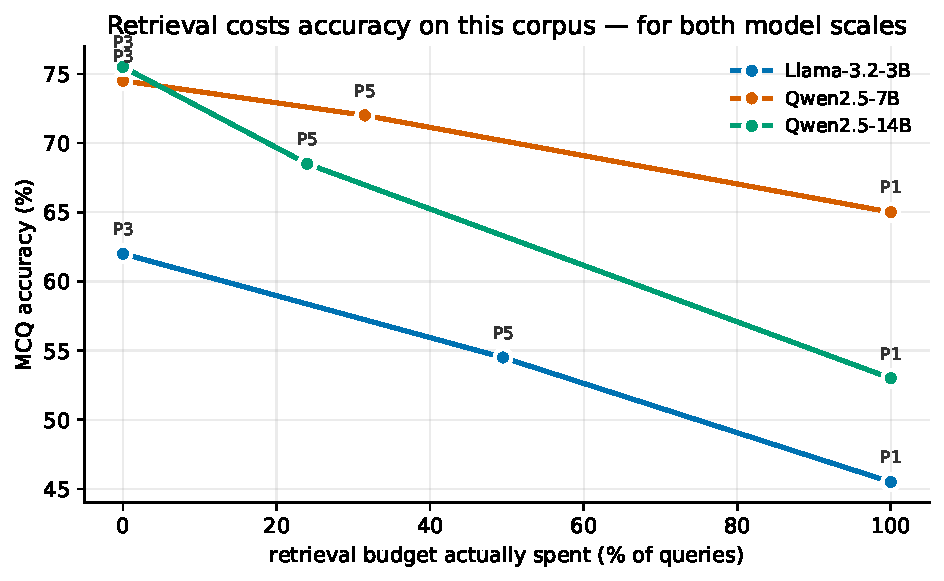
\includegraphics[width=0.8\linewidth]{results/figures/fig_scaling}
  \caption{Multiple-choice accuracy against the retrieval budget actually
    spent. Every model loses accuracy as retrieval increases on this corpus,
    and the larger models sit uniformly higher. The P5 points do not share an
    $x$-position, which is the limitation discussed in
    Section~\ref{sec:scaling-budget}.}
  \label{fig:scaling}
\end{figure}

\section{Closed-Book Capability: A Curve That Flattens}
\label{sec:scaling-closedbook}

Closed-book accuracy is the cleanest cross-model comparison, since no policy
retrieves and no budget confound applies. It rises and then plateaus, at
\accPthreeMcq{} for 3B, \accQwenPthreeMcq{} for 7B and
\accQwenFourteenPthreeMcq{} for 14B. The two steps are not equal, because the
3B-to-7B step adds \scaleGainSmall{}pp while the 7B-to-14B step, across a
model twice the size, adds \scaleGainLarge{}pp. Doubling the parameters a
second time buys almost nothing on this benchmark.

Both models answered the same \mcnemarN{} questions on the first step, so a
paired test is available: \mcnemarBoth{} correct for both, \mcnemarNeither{}
for neither, \mcnemarOnlyQwen{} for Qwen alone and \mcnemarOnlyLlama{} for
Llama alone, giving $\chi^2 = \mcnemarChi{}$ on the discordant pairs, which is
comfortably beyond the $3.84$ threshold for $p < 0.05$. The larger model is
genuinely better, and the \mcnemarOnlyLlama{} questions the smaller model
wins show that scale redistributes competence rather than simply adding it.
From 7B to 14B the aggregate barely moves, which is the more consequential
fact and is taken up in Section~\ref{sec:scaling-bars}.

\section{Selective Beats Always-Retrieve, and at 14B, Significantly}
\label{sec:scaling-selective}

Within each model, where the comparison is legitimate, P5 leads P1 on
multiple-choice at all three scales, by \diffPfivePone{}pp on the 3B,
\diffQwenPfivePone{}pp on the 7B and \diffFourteenPfivePone{}pp on the 14B.
On the two smaller models the 95\% intervals (\diffPfivePoneCI{} and
\diffQwenPfivePoneCI{}) cross zero, so each is individually consistent with an
improvement rather than a demonstration of one. At 14B the interval is
\diffFourteenPfivePoneCI{}, which excludes zero, so the advantage of selective
over always-retrieve is statistically significant on a single model for the
first time in this project. The claim is therefore supported both by three
same-direction estimates whose agreement across scales is itself evidence, and
by one estimate that clears significance on its own.

\section{The Mechanism: Distraction Scales with Capability}
\label{sec:scaling-mechanism}

The paired closed-book-versus-always-retrieve analysis of
Section~\ref{sec:eval-distraction}, repeated at each scale, counts the
multiple-choice questions where always-retrieving breaks a closed-book-correct
answer against those it fixes:

\begin{quote}
  3B: \breakLlama{} broken / \fixLlama{} fixed (\harmRatioLlama{}$\times$)
  \quad 7B: \breakQwenSeven{} / \fixQwenSeven{}
  (\harmRatioQwenSeven{}$\times$) \quad
  14B: \breakQwenFourteen{} / \fixQwenFourteen{}
  (\harmRatioQwenFourteen{}$\times$).
\end{quote}

The fixes never vanish, since the corpus keeps supplying answers the model
lacked at every scale, but the breakages grow and the 14B breaks the most
correct answers of any model. That gradient is the signature of displacement
rather than of a deficient corpus, because a corpus that simply lacked
information would damage a stronger model less, given that a stronger model
can fall back on what it knows, whereas here the strongest model is harmed the
most precisely because it holds the most correct knowledge to be displaced.
Section~\ref{sec:disc-synthesis} develops this into the dissertation's central
reframing and rules out the corpus-absence objection in full. For the scaling
story it is enough that the phenomenon the gate exists to manage strengthens
with scale rather than weakening, which is why always-retrieve is punished
hardest at 14B and why the gap there is wide enough to reach significance.

\section{Open-Ended Questions: Saturation, Then Inversion}
\label{sec:scaling-saturation}

The thresholds refitted in Section~\ref{sec:scaling-nontransfer} were fitted
on multiple-choice drafts, and reusing them unchanged on open-ended drafts
proved unsound.

% AUTO-GENERATED by scripts/generate_tables.py -- DO NOT EDIT.
% Regenerate with: python scripts/generate_tables.py
% Every number is computed from results/raw_logs/ via evaluation.loading.
% git 855a45b | 2026-08-02 01:10
\begin{table}[t]
  \centering
  \small
  \begin{tabular}{lllcc}
    \toprule
    Model / task & Gate & $\tau$ & signal min / med / max & fires \\
    \midrule
    Llama-3.2-3B / MCQ & entropy & 0.700 & 0.200 / 0.718 / 1.532 & 52.0\% \\
     & margin & 0.700 & 0.462 / 0.695 / 0.892 & 53.5\% \\
     & probe & --- & --- (threshold-free) & 40.0\% \\
    \midrule
    Llama-3.2-3B / open & entropy & 0.700 & 0.324 / 0.877 / 1.744 & 75.5\% \\
     & margin & 0.700 & 0.346 / 0.624 / 0.853 & 79.0\% \\
     & probe & 0.700 & 0.071 / 0.509 / 1.000 & 87.0\% \\
    \midrule
    Qwen2.5-7B / MCQ & entropy & 0.187 & 0.000 / 0.241 / 0.960 & 34.5\% \\
     & margin & 0.899 & 0.712 / 0.927 / 1.000 & 40.5\% \\
     & probe & --- & --- (threshold-free) & 7.5\% \\
    \midrule
    Qwen2.5-7B / open (MCQ $\tau$) & entropy & 0.187 & 0.215 / 0.540 / 1.001 & \textbf{100.0\%} \\
     & margin & 0.899 & 0.658 / 0.769 / 0.854 & \textbf{100.0\%} \\
     & probe & 0.700 & 0.077 / 0.538 / 0.836 & 82.9\% \\
    \midrule
    Qwen2.5-7B / open (recalib.) & entropy & 0.568 & 0.050 / 0.554 / 1.119 & 47.0\% \\
     & margin & 0.752 & 0.618 / 0.766 / 0.972 & 39.5\% \\
     & probe & 0.538 & 0.053 / 0.545 / 1.000 & 47.5\% \\
    \midrule
    Qwen2.5-14B / MCQ & entropy & 0.250 & 0.000 / 0.324 / 0.791 & 29.5\% \\
     & margin & 0.861 & 0.551 / 0.921 / 0.999 & 29.0\% \\
     & probe & --- & --- (threshold-free) & 7.5\% \\
    \midrule
    Qwen2.5-14B / open & entropy & 0.536 & 0.138 / 0.514 / 0.929 & 46.0\% \\
     & margin & 0.750 & 0.609 / 0.760 / 0.922 & 43.5\% \\
     & probe & 0.712 & 0.250 / 0.643 / 1.000 & 63.5\% \\
    \bottomrule
  \end{tabular}
  \caption{Gate saturation. The entropy gate fires when its signal exceeds
  $\tau$; the margin and probe gates fire when theirs fall below it. For
  Qwen on open-ended questions the entropy signal's \emph{minimum} lies above
  its threshold and the margin signal's \emph{maximum} lies below its own, so
  every question retrieves and P5 degenerates into P1. Both thresholds were fitted
  on multiple-choice drafts and reused unchanged on open-ended drafts, whose signal
  distributions differ; the probe is threshold-free on MCQ (letter agreement) and
  so reports no range there. Llama saturates less only because its $\tau=0.70$
  happens to fall inside its open-ended distribution.}
  \label{tab:gate-saturation}
\end{table}


The entropy gate votes to retrieve when its signal exceeds $\tau$, and on the
7B's open-ended questions the smallest observed signal,
\qwenOpenEntropyMin{}, already exceeds its threshold of
\qwenOpenEntropyTau{}. The margin gate votes when its signal falls below
$\tau$, and its largest observed signal, \qwenOpenMarginMax{}, lies below its
threshold of \qwenOpenMarginTau{}. Neither gate has a decision to make, so
every question retrieved and P5 was not a selective policy at all but P1
wearing P5's name (Table~\ref{tab:gate-saturation},
Figure~\ref{fig:gate-saturation}). The cause is a distributional shift the
method did not anticipate, since a multiple-choice draft is a single letter
while an open-ended draft is a paragraph of free text, and their signal
distributions barely overlap (Figure~\ref{fig:signal-shift}). The lesson
generalises: \textbf{gate thresholds are task-specific as well as
model-specific}, and a threshold fitted on one question format must not be
deployed on another. Llama escapes total saturation on the same task only
because its $\tau = 0.70$ happens to fall inside its open-ended distribution,
which is luck rather than design, and even then it retrieves at
\retPfiveOpen{}, far above the intended budget. The open-ended gated runs on
both Qwen models were therefore recalibrated on open-ended drafts, using one
global operating point per task type, and it is those runs reported below.

\begin{figure}[t]
  \centering
  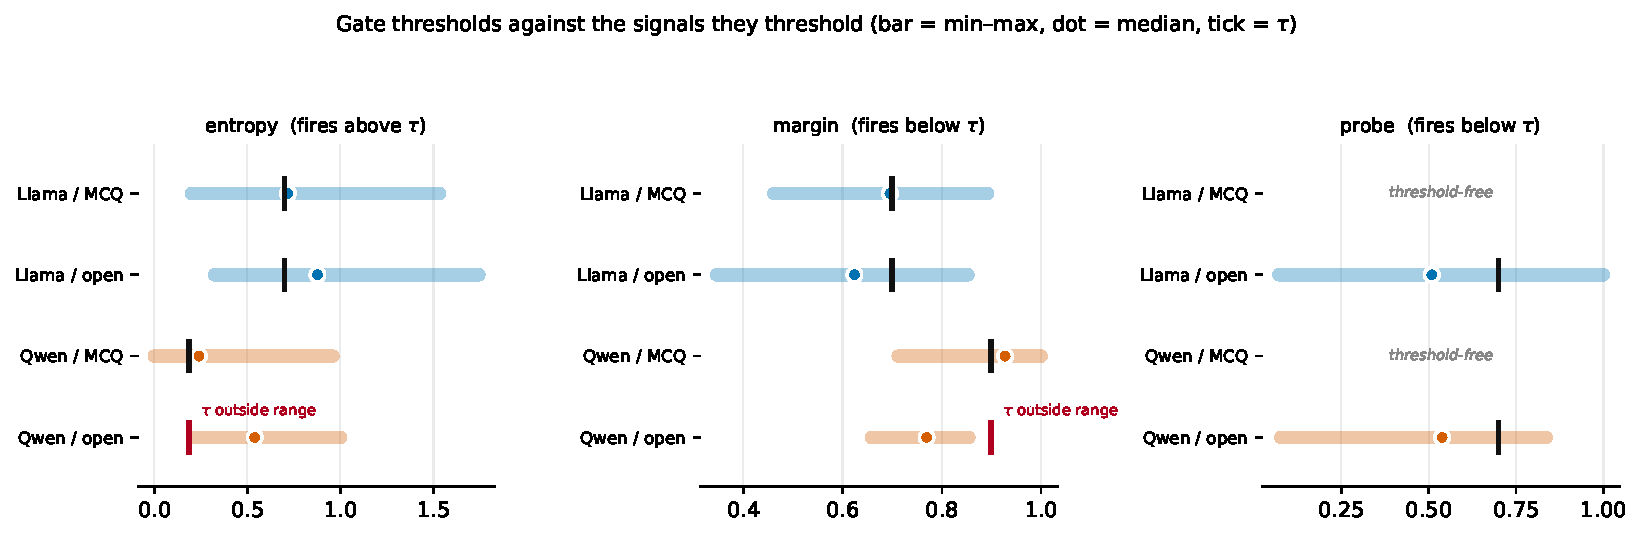
\includegraphics[width=\linewidth]{results/figures/fig_gate_saturation}
  \caption{Each gate's threshold against the distribution of the signal it
    thresholds. A threshold drawn outside its own range bar is a gate with no
    decision to make, and both of the 7B's logit gates are in that state on
    open-ended questions under multiple-choice thresholds.}
  \label{fig:gate-saturation}
\end{figure}

\begin{figure}[t]
  \centering
  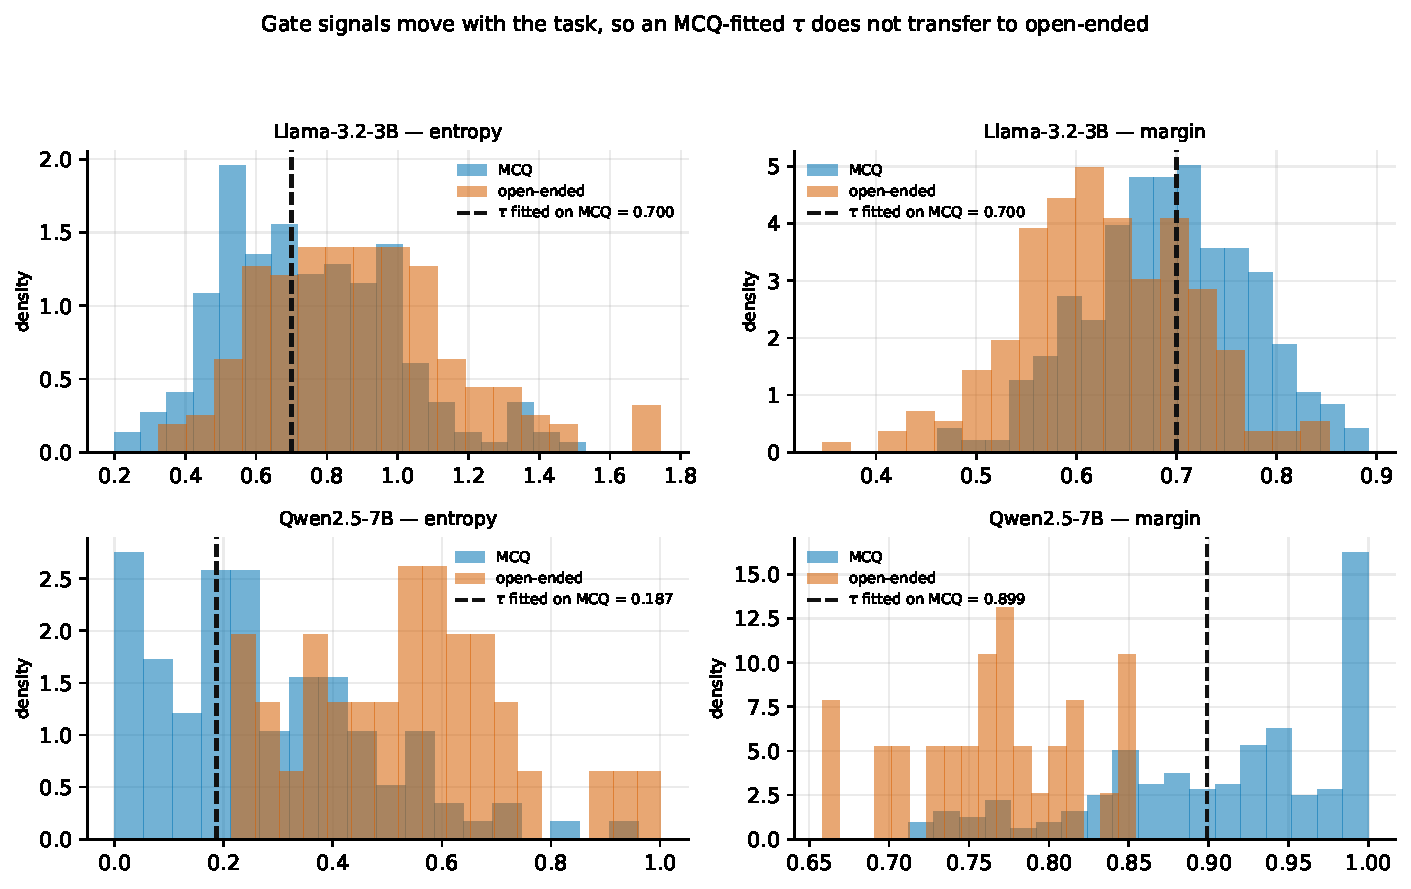
\includegraphics[width=\linewidth]{results/figures/fig_signal_shift}
  \caption{Gate-signal distributions for the same model and the same gate on
    multiple-choice versus open-ended questions, with the multiple-choice
    threshold overlaid. The distributions barely overlap, which is why a
    threshold fitted on one lands in the wrong part of the other.}
  \label{fig:signal-shift}
\end{figure}

With the gates functioning, the open-ended arm is complete at $n=200$ for
every policy and model, and the finding lies in the ordering of the three
policies and how it changes with scale:

\begin{quote}
  \textbf{3B:} P1 (\fOnePoneOpen{}) $>$ P5 (\fOnePfiveOpen{}) $>$ P3
  (\fOnePthreeOpen{}), so always-retrieve is best and retrieval helps.\\
  \textbf{7B:} P3 (\fOneQwenPthreeOpen{}) $>$ P5 (\fOneQwenPfiveOpen{})
  $>$ P1 (\fOneQwenPoneOpen{}), so closed-book is best and retrieval hurts.\\
  \textbf{14B:} P3 (\fOneQwenFourteenPthreeOpen{}) $>$ P5
  (\fOneQwenFourteenPfiveOpen{}) $>$ P1 (\fOneQwenFourteenPoneOpen{}), the
  same inverted order as 7B.
\end{quote}

The ordering inverts between the smallest model and the larger two and then
holds. On the 3B, open-ended research questions sit outside the model's
parametric knowledge, so retrieved context is a net help, whereas by 7B the
model already knows more than the passages reliably add and the same corpus
that helped now hurts, and at 14B the inversion persists unchanged. The
reversal is therefore a stable property of the two larger models rather than a
quirk of the 7B, which is the strongest form the observation can take without
a fourth scale. Open-ended questions are simply where parametric knowledge
runs out last, so the retrieval-hurts regime that multiple-choice showed at
every scale reaches open-ended only once the model is large enough. Two
cautions bound these rows, which are that open-ended budgets are not matched
across models, so the P5 figures are ordinal positions within each model's own
P1 to P3 range, and that paragraph-level token-$F_1$ is surface-lexical, so
only orderings are interpreted and never the size of a gap.

\section{Scale Versus the Safety Bars}
\label{sec:scaling-bars}

The most consequential cross-model fact is where the curve sits relative to
the clinical bars (\barLow{}/\barMedium{}/\barHigh{}). The 3B cleared none.
Both Qwen models clear the \barLow{} low-risk bar on their best policy, at
\accQwenPthreeMcq{} and \accQwenFourteenPthreeMcq{}, so the safety envelope
that was empty at 3B is populated at low risk once capability is sufficient.
Neither larger model reaches the \barMedium{} medium-risk bar, however, and
the curve is flattening as it approaches, since the \scaleGainLarge{}pp gained
from 7B to 14B is a twelfth of the \scaleGainSmall{}pp gained from 3B to 7B.
Extrapolating to the medium-risk bar would require a scale increase that the
measured diminishing returns give no reason to expect would be enough.

This is the result that most sharpens the dissertation's argument. Scaling is
a real lever, since it moved the system from clearing no bar to clearing the
low one, but it is a saturating lever and it saturates below the threshold
that medium-risk clinical use would demand. That is precisely the regime in
which method matters, because if raw capability cannot be scaled to safety
within a practical range, then the discipline of retrieving only when it helps
becomes part of how the remaining distance has to be closed rather than an
efficiency nicety. Two further results point the same way. The closed-book
curve plateaus sharply after 7B, so using a bigger model is a weaker remedy
than it first appears, and the open-ended retrieval-helps result from the 3B
did not merely fail to replicate but inverted and then held inverted at 14B.
Taken together they say that the value of retrieval is a function of the gap
between what the model knows and what the passages add, which scaling closes
on the tasks the model can already do, and which the gate exists to detect on
the tasks it cannot.

Latency is not comparable across all three models, because the 3B ran on CPU
and both Qwen models on a T4 GPU, so a three-way comparison would measure the
accelerator rather than the model. The within-GPU comparison is clean, with
closed-book answering a multiple-choice question in \latQwenPthreeMcq{} at 7B
and \latQwenFourteenPthreeMcq{} at 14B against \latQwenPfiveMcq{} and
\latQwenFourteenPfiveMcq{} for the gated policy. The gate's cost is the price
of its extra draft generations, it scales gently with model size, and it
remains within an interactive budget, so cost does not disturb the accuracy
conclusions.